\label{marco_teo}

En este capítulo se describirá el modelo en el cual se basa toda la investigación, también se definirán los conceptos utilizados a lo largo del trabajo como la definición de la presión social y los "blocking clusters". Además se comentará el algoritmo de integración temporal utilizado en la evolución temporal de cada proceso. 

\section{\label{sfm}Modelo de Fuerza social}

El modelo de "fuerza social" básico considera a los individuos como partículas auto-impulsadas. El movimiento de de los individuos está dominado por tres tipos de fuerzas, de naturaleza diferente: la fuerza de deseo (autopropulsión), fuerzas sociales (repulsión) y fuerzas granulares (rozamiento).  \\

La fuerza de deseo expresa el hecho de que cada persona es capaz de  acelerar o desacelerar hasta alcanzar la velocidad en que se siente más cómoda. La magnitud de esta velocidad se corresponde con el nivel de ansiedad que tenga por llegar a un cierto lugar. La expresión matemática de esta fuerza viene dada por la fórmula~\ref{fdeseo}. Esta fórmula refleja el hecho que el individuo i-esimo que posee masa $m_i$, desea  moverse con una velocidad $v_d^ {(i)}(t)$ en una dirección $\hat{\mathbf{e}}_d^ {(i)}(t)$, por lo tanto readapta su velocidad $\mathbf{v}_i(t)$ con un cierto tiempo característico $\tau$.
\begin{equation}
\mathbf{f}_d^ {(i)}(t)=m_i\,\displaystyle\frac{v_d^ {(i)}(t)\,\hat{\mathbf{e}}_d^ {(i)}(t)-\mathbf{v}_i(t)}{\tau}\label{fdeseo}
\end{equation}

La repulsión social es una fuerza que describe la tendencia que tienen las personas a mantenerse alejadas unas de otras. Depende de la distancia de separación entre individuos $d_{ij}=\left\|\mathbf{r_i}-\mathbf{r_j}\right\|$ y está en la dirección normal $\mathbf{n}_{ij}=(\mathbf{r_i}-\mathbf{r_j})/d_{ij}$ (versor que apunta desde el individuo j al individuo i). Los peatones están en contacto si el valor de $d_{ij}$ es más chico que la suma de los radios $r_{ij}=(r_i+r_j)$. $A_i$ y 	$B_i$ son constantes que se determinan experimentalmente.

\begin{equation}
\mathbf{f}_s^{(ij)}=A_i\,e^{(r_{ij}-d_{ij})/B_i}\mathbf{n}_{ij}\label{fsocial}
\end{equation} 

Cuando los individuos están en contacto, comienza a actuar una fuerza de rozamiento, la misma es proporcional a la velocidad relativa entre los mismos $\Delta \mathbf{v}_{ij}=(\mathbf{v}_i-\mathbf{v}_j)$. La dirección tangencial está representada por $\mathbf{t}_{ij}=(-n_{ij}^2,n_{ij}^1)$.  $\kappa$ es una constante y $g(x)$ es una función nula cuando los individuos no se tocan $(r_{ij}<d_{ij})$ y toma el valor de su argumento en caso contrario. 
\begin{equation}
\mathbf{f}_g^{(ij)}=\kappa\,g(r_{ij}-d_{ij})\,\Delta \mathbf{v}_{ij}\cdot\mathbf{t}_{ij}\label{frozamiento}
\end{equation}

Se trata de forma análoga a la interacción de los individuos con las paredes. $d_{iW}$ es la distancia del i-esimo peatón con la pared W, $n_{iW}$ la dirección perpendicular entre éstos y $t_{iW}$ la tangencial. La expresión (\ref{fparedes}) agrupa tanto a la repulsión como al rozamiento de la interacción peatón-pared.

\begin{equation}
\mathbf{f}^{iW}=A_ie^{(r_{i}-d_{iW})/B_i}\mathbf{n}_{iW}-\kappa g(r_{i}-d_{iW})\Delta \mathbf{v}_{i}\cdot\mathbf{t}_{iW}
\label{fparedes}
\end{equation} 

Con todo esto, mediante la fórmula (\ref{newton}), puede expresarse la variación de velocidad en el tiempo que siente un individuo. $f^{ij}$ es el término de interacción entre individuos, es la suma de la repulsión y el rozamiento. El cambio de posición viene dado por $v_{i}(t)=d\mathbf{r_i}/dt$.

\begin{equation}
m_i\frac{d\mathbf{v_i}}{dt}=\mathbf{f}_d^ {(i)}(t)+ \sum_{i\neq j}^{N}\mathbf{f}^{(ij)} + \sum_{W}^{N}\mathbf{f}^{(iW)}
\label{newton}
\end{equation}  

Uno de los resultados más trascendentes de este modelo es el efecto "Faster is slower" \cite{Helbing1}. A partir de cierto grado de ansiedad ($v_d=2$~m/s) un incremento en la velocidad de deseo produce evacuaciones menos eficientes (los peatones tardan más en evacuar). 
 
\section{Presión local}

A pesar de que la fuerza de deseo es una fuerza unilateral (\textit{i.e.} partícula auto-impulsada), la ecuación de movimiento continúa siendo válida, y por lo tanto, podemos derivar la relación del virial\cite{lion}.

\begin{equation}
 \bigg\langle\displaystyle\sum_{i=1}^N\displaystyle\frac{p_i^2}{m_i} + 
\displaystyle\sum_{i=1}^N 
\mathbf{r}_i\cdot\mathbf{f}_i\bigg\rangle=-3\mathcal{PV}\label{virial1}
\end{equation}


\noindent Para un conjunto de $N$ peatones dentro del volumen $\mathcal{V}$. $p_i$  y $\mathbf{f}_i$ son el momento y la fuerza total actuando sobre el individuo $i$. La fuerza $\mathbf{f}_i$ no contempla la interacción con las paredes.  $\langle\cdot\rangle$ corresponde al valor medio en el tiempo. El lado derecho de la ecuación $-3\mathcal{PV}$ es la presión global en la superficie del recinto $\mathcal{V}$.  \\
% El término de la derecha es negativo porque se considera a la fuerza que la pared ejerce sobre el individuo. 
La presión local para un peatón ($i$) está asociada a las fuerzas (por unidad de área) actuando sobre él debidas a los individuos que lo rodean. Según Ref.~\cite{lion} se puede definir una "función de presión social" $P_i$ como:\\

\begin{equation}
3P_iV_i=\displaystyle\frac{p_i^2}{m_i} + \frac{1}{2}
\displaystyle\sum_{j=1}^{N-1}
\mathbf{r}_{ij}\cdot\mathbf{f}_s^{(ij)}\label{pv}
\end{equation}

\noindent donde $V_i$ es el volumen que encierra al peatón $i$ y 
$\mathbf{r}_{ij}=\mathbf{r}_{i}-\mathbf{r}_j$ (la distancia
entre dos peatones en la dirección desde j hacia i). Cabe destacar que el producto interno $\mathbf{r}_{ij}\cdot\mathbf{f}_s^{(ij)}$ siempre es positivo debido a la repulsión y es igual al producto escalar (positivo) $d_{ij}f_s^{(ij)}$. El factor 1/2 evita el doble conteo de las interacciones cuando se hace la suma de todos los $3P_iV_i$ \\ 

El segundo término en la ecuación (\ref{virial1}) puede dividirse en la suma de productos internos $\mathbf{r}_i\cdot\mathbf{f}_d$ (deseo), 
$\mathbf{r}_i\cdot\mathbf{f}_s$ (social) y $\mathbf{r}_i\cdot\mathbf{f}_g$ (granular). De hecho, la suma del producto social depende de la distancia entre partículas $d_{ij}f_s^{(ij)}$, mientras que la parte granular no tiene ningún rol por su ortogonalidad ($\mathbf{r}_{ij}\cdot\mathbf{f}_g^{(ij)}=0$). Por lo tanto, la relación del virial (\ref{virial1}) se expresa \\  

\begin{equation}
 \displaystyle\sum_{i=1}^N\langle3P_iV_i 
\rangle=-3\mathcal{PV} -\displaystyle\sum_{i=1}^N \langle
\mathbf{r}_i\cdot\mathbf{f}_d^{(i)}\rangle\label{virial2}
\end{equation}

Hay que destacar que la ecuación (\ref{virial2}) se cumple si los peatones están en contacto o no. Esto significa que no se trata de una presión de contacto (habitual en los sistemas físicos tradicionales) sino de una presión que provoca una cambio en el patrón de movimiento del individuo.\\

La suma de fuerzas por unidad de circunferencia (\textit{i.e.} medida de presión según la Ref.~\cite{Helbing1}) es similar a la definición dada en (\ref{pv}) y que, a su vez, se sigue de la Ref.\cite{lion}. Comprobamos durante la investigación que ambas son proporcionales (no mostrado en este trabajo).\\   

En la Ref.~\cite{Helbing1} se reporta que a valores de presión superiores a 1600 Nm$^{-1}$ los individuos se lastiman y se vuelven obstáculos inamovibles. En este trabajo no se tienen en cuenta los eventuales desmayos producidos por las altas presiones. 

\section{Blocking Clusters}

Se utilizó el concepto de blocking cluster~\cite{Dorso1} para estudiar a los individuos más próximos a la puerta que satisfacen la condición de estar en contacto con ella.
Se lo define como un conjunto mínimo de individuos en contacto que va desde un punto de la pared hacia otro. Estos puntos están próximos a los costados de la puerta. Aquellos peatones que conforman el blocking cluster son los responsables de bloquear la salida. Típicamente los blocking cluster formados en las evacuaciones tiene estructura de "arco" como el que se muestra en la Fig. \ref{bc}. Basta que un solo peatón deje de estar en contacto con sus vecinos para que el blocking cluster deje de estar constituido. Además, estas estructuras mínimas actúan como una barrera para los individuos que tienen detrás, impidiendo la evacuación de peatones. \\

En este trabajo consideramos dos definiciones adicionales referentes a los \textit{blocking clusters}: por un lado, si éste no está en contacto con la pared de separación entre las puertas (pero sí con las otras paredes del mismo lado del recinto) lo llamamos \textit{big blocking cluster}. En cambio, si una de las paredes de contacto es la pared de separación entre puertas, entonces los llamamos \textit{small blocking cluster} (ver ejemplos en la Fig.~\ref{bc}).

\begin{figure}[H]
    \centering
    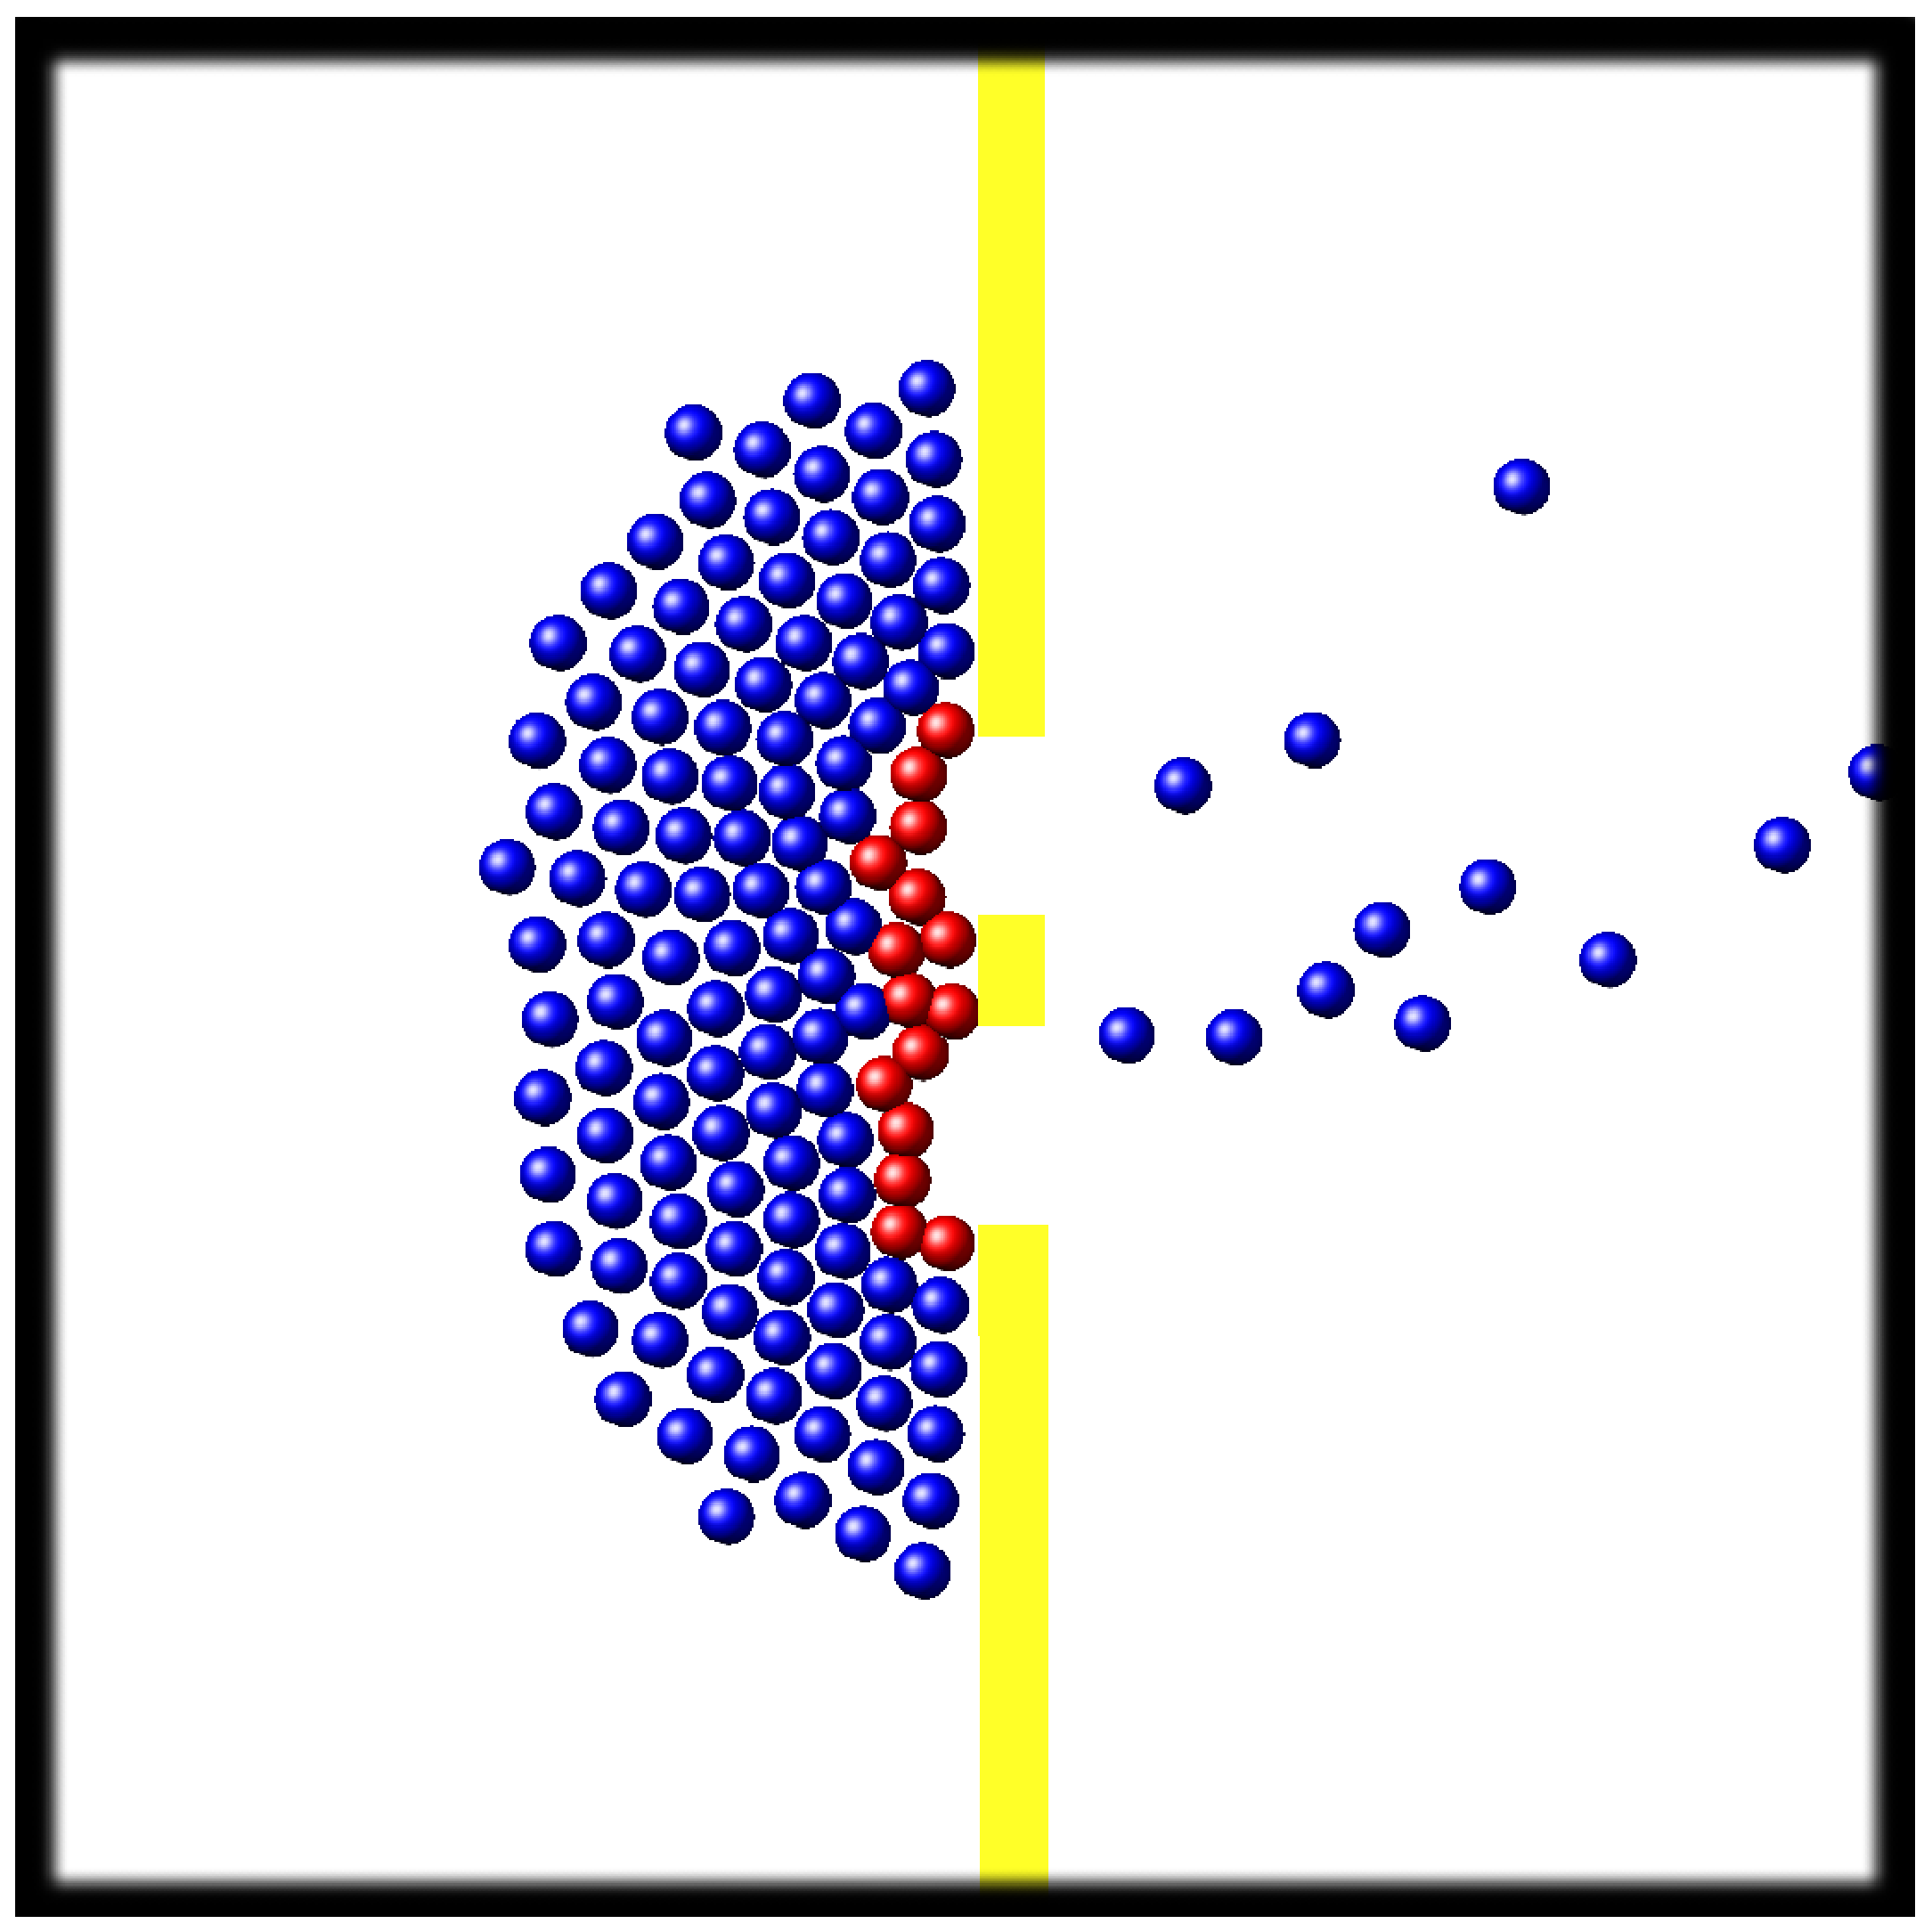
\includegraphics[width=7cm]{figuras/big_bc.eps}
    \hfill
    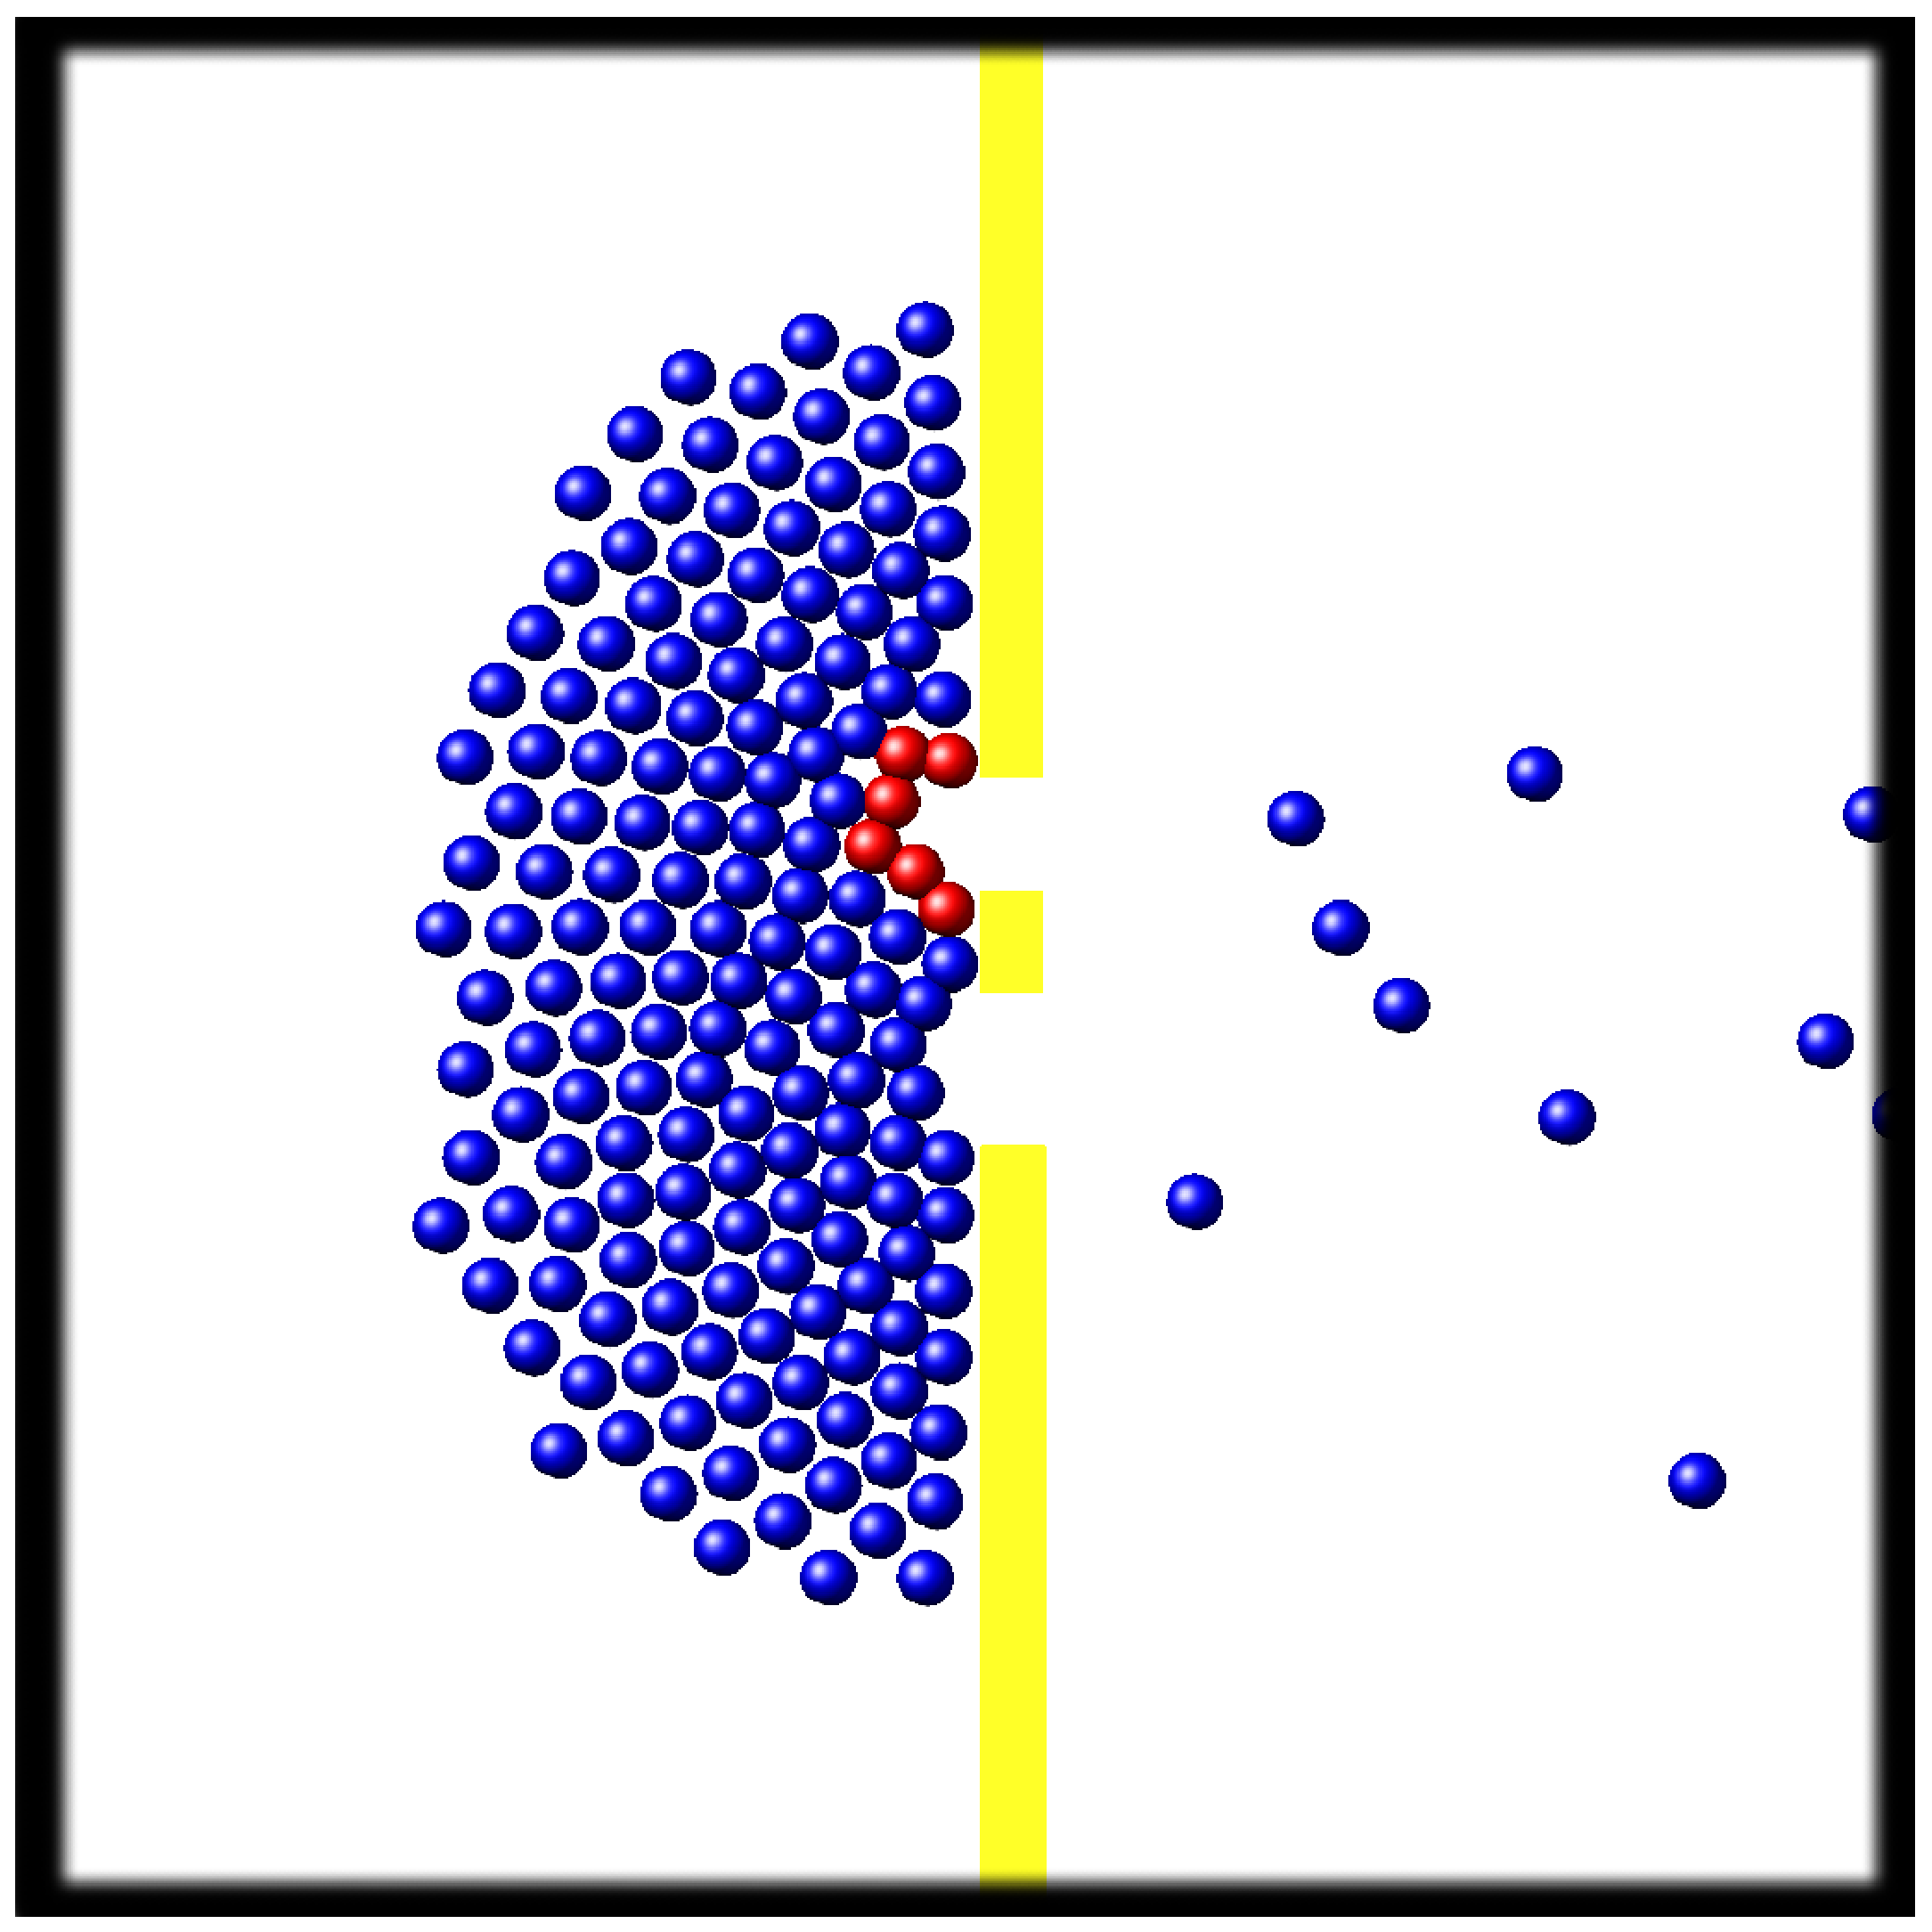
\includegraphics[width=7cm]{figuras/small_bc.eps}
    \caption[width=5cm]{Imagen del proceso de evacuación de  200 individuos a través de dos puertas (velocidad de deseo $v_d=4\,$m/s). Las paredes se muestran en amarillo. Los inidividuos corresponden a las partículas en color azul. La salida de personas se produce de izquierda a derecha. Los \textit{blocking clusters} están identificados en color rojo. (a) se muestra un \textit{big blocking cluster}. Ningún individuo está en contacto con la pared de seperación entre puertas. (b)  Se muestra un \textit{small blocking cluster} alrededor de la puerta superior.}
    \label{bc}
\end{figure}


\section{Algoritmo de Verlet}

Para integrar las ecuaciones de movimiento se usó el algoritmo de Verlet en velocidades~\cite{haile}. Este método es ampliamente utilizado en el campo de dinámica molecular.En esta forma de resolución la posición y velocidad son calculados en el mismo paso temporal. Las ecuaciones que lo describen son:

\begin{equation}
x(t+\Delta t)=x(t)-v(t)\Delta t + \frac{1}{2}a(t)\Delta t^2 
\label{verlet_x}
\end{equation} 

\begin{equation}
v(t+\Delta t)=v(t)+\frac{a(t)+a(t+\Delta t)}{2}\Delta t
\label{verlet_v}
\end{equation}

El esquema de Verlet tiene un error de truncamiento local de ($\Delta t^2$). En la Fig. \ref{esquema_verlet} se muestra un diagrama del procedimiento, en donde se detalla la secuencia de actualización de variables para cada individuo. En el estado inicial disponemos únicamente de las posiciones y las velocidades de los individuos. Las aceleraciones se obtienen por medio de evaluación de las fuerzas $\mathbf{f}_d$, $\mathbf{f}_s$ y $\mathbf{f}_g$. Con estas magnitudes 
se calcula una nueva posición, se re-evalúan las fuerzas (aceleraciones) y se re-calcula la velocidad. Luego se vuelven a actualizar la posiciones y se repite el ciclo hasta construir las trayectorias de las partículas.
En la sección \ref{ci} del capítulo \ref{simulaciones} se detallarán las condiciones iniciales usadas en cada proceso de evacuación.\\

El algoritmo de Verlet es ampliamente utilizado por preservar las simetrías de las ecuaciones de newton y las propiedades físicas de una gran cantidad de sistemas. Esto es gracias al hecho que tiene reversibilidad temporal y es simpléctico (preserva el volumen en el espacio de fases). Además, es simple de implementar y posee buena estabilidad incluso para pasos temporales moderadamente grandes.

\begin{figure}[H]
    \centering
        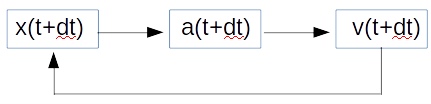
\includegraphics[scale=0.7]{figuras/esquema_verlet.png}
    \caption[width=5cm]{Esquema del procedimiento algorítmico de Verlet en velocidades}
    \label{esquema_verlet}
\end{figure}
